\chapter{Les systèmes sensoriels}\label{ch:b3:sensory-systems}

Par nuit noire un œil humain sait détecter un éclair de quelques
photons --- la plus petite quantité de lumière que la physique permette
de détecter. L'oreille entend un son qui déplace le tympan de moins que
le diamètre d'un atome d'hydrogène, et distingue un ton d'un autre qui
en diffère d'un cinquième de pour cent. Un chien suit une piste de
quelques molécules par centimètre cube~; un requin trouve un poisson
plat sous le sable au champ électrique de ses battements de cœur. Chaque
sens commence par une cellule qui convertit une forme d'énergie en une
variation de potentiel de membrane, et chaque sens finit en potentiels
d'action dans un nerf~; entre les deux se tiennent les problèmes que
traite ce chapitre~: comment un récepteur amplifie une seule molécule ou
un seul photon en un signal qu'un neurone puisse lire, comment une
étendue d'un facteur mille milliards en intensité se comprime en une
fréquence de quelques centaines de potentiels par seconde, comment une
onde mécanique est triée par fréquence, comment dix mille odeurs se
distinguent avec quatre cents récepteurs, et comment le cerveau, qui ne
reçoit jamais que des potentiels, sait de quel sens ils viennent.

\section{Les principes communs à tous les sens}

\begin{definition}[Transduction, codage et adaptation]\label{def:b3:sensory-systems:principles}
\index{transduction sensorielle}\index{potentiel de récepteur}\index{ligne étiquetée}\index{champ récepteur}\index{adaptation!sensorielle}\index{inhibition latérale}
Une \emph{cellule réceptrice sensorielle} contient un mécanisme de
\emph{transduction} --- une protéine ou une cascade --- qui convertit un
stimulus (un photon, une molécule, un déplacement, de la chaleur, un
champ électrique) en une variation de conductance de la membrane et donc
en un \emph{potentiel de récepteur}, gradué avec le stimulus~; la
cellule, ou le neurone sur lequel elle fait synapse, en fait un train de
potentiels d'action dont la fréquence code l'intensité. La
\emph{modalité} d'un signal n'est pas donnée par les potentiels, qui
sont identiques dans tous les nerfs, mais par le fil qu'ils empruntent
et par l'endroit du cerveau où il aboutit~: une \emph{ligne étiquetée}.
Un neurone sensoriel répond aux stimulus d'un \emph{champ récepteur} ---
une plage de peau, une région du champ visuel, une bande de fréquences
--- et les champs voisins s'affinent l'un l'autre par
\emph{inhibition latérale}, chaque neurone étouffant ses voisins de
sorte que bords et contrastes sont exagérés. La plupart des récepteurs
s'\emph{adaptent}~: leur réponse à un stimulus maintenu décline, de
sorte qu'ils rapportent le changement plutôt que le niveau, et leur
plage de travail se déplace pour se poser autour du fond ambiant.
\end{definition}

\begin{theorem}[Weber, Fechner et Stevens]\label{thm:b3:sensory-systems:weber}
\index{loi de Weber}\index{loi de Fechner}\index{loi de puissance de Stevens}
L'observation de Weber (1834) est que le plus petit changement
détectable $\Delta I$ dans un stimulus d'intensité $I$ en est une
fraction fixe~: $\Delta I/I = k$, avec $k$ valant environ $0.02$ pour le
poids, $0.08$ pour la clarté, $0.1$ pour la force sonore. Si chaque
différence juste perceptible compte pour une unité de sensation $S$,
alors $\mathrm{d}S = \mathrm{d}I/
(kI)$ et
\[
S = \frac{1}{k}\ln\frac{I}{I_{0}} ,
\]
où $I_{0}$ est le seuil~: la sensation croît comme le logarithme du
stimulus (Fechner, 1860), et c'est pourquoi les intensités se mesurent
en \omterm{def:b3:sensory-systems:cochlea}{décibels} et en magnitudes, et pourquoi une bougie ajoutée à une
bougie se remarque et une bougie ajoutée à un projecteur non. Les
expériences d'échelle directe, où les sujets attribuent des nombres aux
sensations, donnent plutôt une loi de puissance $S \propto I^{n}$
(Stevens, 1957), avec $n \approx
0.3$ pour la force sonore et la clarté, $1$ pour la longueur d'un trait
et $3.5$ pour le choc électrique~; un logarithme et une petite puissance
sont presque indiscernables sur quelques décades, et les deux lois
s'accordent sur l'essentiel~: le système nerveux comprime.
\end{theorem}
\begin{proof}
De $\Delta I = kI$ pour une unité de $S$, l'accroissement de sensation
par accroissement de stimulus vaut $\mathrm{d}S/\mathrm{d}I = 1/(kI)$~;
en intégrant depuis le seuil $I_{0}$, où $S = 0$, on obtient $S = (1/k)
\ln(I/I_{0})$. La loi de puissance est l'hypothèse de rechange selon
laquelle un \emph{rapport} fixe de stimulus produit un \emph{rapport}
fixe de sensations, $\mathrm{d}S/S = n\,\mathrm{d}I/I$, dont l'intégrale
est $S \propto I^{n}$~; pour $n \to 0$ avec un changement d'échelle
convenable elle tend vers le logarithme.
\end{proof}

\begin{omfigure}
\begin{tikzpicture}
\begin{axis}[
  width=0.68\linewidth, height=5.6cm,
  xmode=log,
  xmin=1, xmax=1e6, ymin=0, ymax=15,
  xlabel={intensité du stimulus $I/I_{0}$}, ylabel={sensation $S$ (unités arbitraires)},
  xlabel style={font=\small, at={(axis description cs:0.5,-0.12)}, anchor=north}, ylabel style={font=\small},
  tick label style={font=\small}, ytick={0,5,10,15},
  clip=false,
]
\addplot[very thick, omDef, domain=1:1e6, samples=100] {ln(x)};
\addplot[very thick, omThm, domain=1:1e6, samples=100] {0.235*x^0.3 - 0.235};
\addplot[very thick, omMeth!70!black, domain=1:1e6, samples=100] {0.5*x^0.24 - 0.5};
\node[font=\scriptsize, omDef, anchor=north west] at (axis cs:2,10.2) {Fechner~: $S = \ln(I/I_{0})$};
\node[font=\scriptsize, omThm, anchor=south east] at (axis cs:9e5,0.4) {Stevens~: $S \propto I^{0.3}$};
\node[font=\scriptsize, omMeth!70!black, anchor=north west] at (axis cs:2,12.5) {Stevens~: $S \propto I^{0.24}$};
\end{axis}
\end{tikzpicture}

{\small La compression d'une étendue d'intensité d'un facteur un million
en une sensation qui croît lentement~: le logarithme de Fechner et les
\omterm{thm:b3:sensory-systems:weber}{lois de puissance de Stevens} à petits exposants sont difficiles à
distinguer sur quelques décades, et toutes deux disent que les sens
rapportent des rapports, non des différences.}
\end{omfigure}

\section{La vision}

\begin{definition}[La rétine]\label{def:b3:sensory-systems:retina}
\index{rétine}\index{bâtonnet}\index{cône}\index{phototransduction}\index{rhodopsine}\index{cellule ganglionnaire}\index{centre--pourtour}
La \emph{rétine} est un feuillet de cerveau au fond de l'œil, trois
couches de cellules avec les photorécepteurs, paradoxalement, au fond,
contre l'épithélium pigmentaire. Les \emph{bâtonnets} --- $10^{8}$ par
œil, un seul pigment, la \emph{rhodopsine} --- servent la faible lumière
et saturent en plein jour~; les \emph{cônes} --- $6\times 10^{6}$, trois
pigments culminant dans le bleu, le vert et le rouge, entassés dans la
fovéa --- servent le jour, la couleur et l'acuité. La
\emph{phototransduction} est une cascade~: un photon isomérise le
chromophore rétinal d'une rhodopsine~; la rhodopsine activée allume des
centaines de molécules de la protéine~G transducine, dont chacune active
une phosphodiestérase qui détruit le GMP cyclique~; la chute du GMPc
ferme les canaux cationiques que le GMPc tenait ouverts dans le noir, le
«~courant d'obscurité~» entrant s'arrête, et la cellule
s'\emph{hyperpolarise} --- la lumière éteint un photorécepteur, qui
libère moins de glutamate. Dans le noir la cellule est dépolarisée et
libère continuellement. Le signal passe aux \emph{cellules bipolaires}
(de types ON et OFF, qui l'inversent ou le conservent) puis aux
\emph{cellules ganglionnaires}, un million par œil, dont les axones
forment le nerf optique --- une compression d'un facteur cent. Les
cellules horizontales et amacrines connectent latéralement, et leur
inhibition donne à chaque cellule ganglionnaire un \omterm{def:b3:sensory-systems:principles}{champ récepteur}
\emph{centre--pourtour}~: excitée par la lumière d'un disque central et
inhibée par celle de l'anneau qui l'entoure (ou l'inverse), de sorte que
la rétine rapporte le contraste local et les bords plutôt que la lumière
absolue.
\end{definition}

\begin{omfigure}
\begin{tikzpicture}[every node/.style={font=\scriptsize}, >=stealth]
  % cascade boxes with amplification numbers
  \node[draw, thick, rounded corners, fill=omProp!30, align=center] (ph) at (0,0) {1 photon};
  \node[draw, thick, rounded corners, fill=omDef!20, align=center] (rh) at (2.6,0) {1 rhodopsine*\\(métarhodopsine II)};
  \node[draw, thick, rounded corners, fill=omDef!20, align=center] (tr) at (5.6,0) {$\sim 500$ transducines\\activées};
  \node[draw, thick, rounded corners, fill=omDef!20, align=center] (pde) at (8.6,0) {$\sim 500$ PDE actives~:\\$\sim 10^{5}$ GMPc hydrolysés};
  \node[draw, thick, rounded corners, fill=omThm!20, align=center] (ch) at (5.6,-2.0) {$\sim 200$ canaux cationiques se ferment~;\\le courant d'obscurité chute de \qty{1}{pA}};
  \node[draw, thick, rounded corners, fill=omMeth!25, align=center] (out) at (1.4,-2.0) {hyperpolarisation de \qty{1}{mV}~;\\moins de glutamate libéré};
  \draw[->, thick] (ph) -- (rh); \draw[->, thick] (rh) -- (tr); \draw[->, thick] (tr) -- (pde);
  \draw[->, thick] (pde.south) |- (ch.east); \draw[->, thick] (ch) -- (out);
  \node[below, font=\tiny, align=center] at (7.1,-2.8) {chaque étape multiplie~; toute la cascade est éteinte en \qty{200}{ms} par\\la rhodopsine kinase, l'arrestine et la GTPase de la transducine, puis remise à zéro};
\end{tikzpicture}

{\small La \omterm{def:b3:sensory-systems:retina}{phototransduction} comme amplificateur. Un photon absorbé
ferme des centaines de canaux par deux étages catalytiques, un gain
d'environ un million en molécules --- assez pour qu'un photon unique
produise un courant mesurable dans un \omterm{def:b3:sensory-systems:retina}{bâtonnet}.}
\end{omfigure}

\begin{theorem}[Compter les photons~: la fréquence de vision]\label{thm:b3:sensory-systems:hecht}
\index{détection d'un photon unique}\index{courbe de fréquence de vision}\index{Poisson!comptage de photons}
Un éclair qui délivre en moyenne $a$ photons absorbés à une plage de
\omterm{def:b3:sensory-systems:retina}{bâtonnets} en délivre, à chaque présentation, un nombre $k$ qui suit une
loi de Poisson~: $P(k) = e^{-a}a^{k}/k!$. Si l'observateur déclare voir
l'éclair dès qu'au moins $n$ photons sont absorbés, la probabilité de
voir vaut
\[
P_{\text{vu}}(a) = 1 - \sum_{k=0}^{n-1} e^{-a}\,\frac{a^{k}}{k!} ,
\]
courbe qui monte de $0$ à $1$ quand $a$ croît, et dont la
\emph{raideur} sur une échelle logarithmique de $a$ ne dépend que de
$n$~: plus le compte seuil est grand, plus la courbe est raide. Ajuster
la courbe mesurée de fréquence de vision donne donc $n$ sans savoir
combien des photons délivrés ont été réellement absorbés.
\end{theorem}
\begin{proof}
Les photons d'une source faible et stable arrivent indépendamment au
hasard, et le nombre absorbé dans un éclair bref de moyenne $a$ suit une
loi de Poisson (limite d'une binomiale à beaucoup de photons chacun
absorbé avec une petite probabilité). Voir demande $k \ge n$, dont la
probabilité vaut un moins la somme des $n$ premiers termes de Poisson.
Multiplier la source par un facteur $c$ multiplie $a$ par $c$ et
translate la courbe le long de l'axe des $\log a$ sans changer sa forme,
de sorte que la forme identifie $n$~: pour $n =
1$, $P = 1 - e^{-a}$ monte sur deux décades de $a$~; pour $n = 6$ elle
monte sur moins d'une.
\end{proof}

\begin{proof}[Faits expérimentaux]
Hecht, Shlaer et Pirenne (1942) firent asseoir des observateurs dans le
noir une demi-heure, puis éclairèrent d'un minuscule point vert, pendant
une milliseconde, la périphérie de la \omterm{def:b3:sensory-systems:retina}{rétine} riche en \omterm{def:b3:sensory-systems:retina}{bâtonnets}, des
centaines de fois à plusieurs intensités, et notèrent la fraction
d'éclairs vus. L'éclair au seuil contenait, à la cornée, quelque $90$
photons, dont (après réflexion, absorption dans les milieux de l'œil et
compte tenu de la chance de $20\,\%$ qu'un photon parvenu à un \omterm{def:b3:sensory-systems:retina}{bâtonnet}
soit absorbé par la \omterm{def:b3:sensory-systems:retina}{rhodopsine}) $5$ à $14$ étaient absorbés. Les \omterm{thm:b3:sensory-systems:hecht}{courbes
de fréquence de vision} avaient la raideur de
$n = 5$ à $7$~: l'observateur disait «~oui~» quand environ six
\omterm{def:b3:sensory-systems:retina}{bâtonnets}, sur les cinq cents situés sous le point, avaient chacun
attrapé un photon unique. Un \omterm{def:b3:sensory-systems:retina}{bâtonnet} détecte un photon~; le cerveau en
exige quelques-uns en coïncidence, pour tenir les fausses alarmes dues
aux isomérisations spontanées des \omterm{def:b3:sensory-systems:retina}{bâtonnets} --- une par \omterm{def:b3:sensory-systems:retina}{bâtonnet} toutes
les quarante secondes --- sous le régime des étoiles.
\end{proof}

\begin{omfigure}
\begin{tikzpicture}
\begin{axis}[
  width=0.68\linewidth, height=5.6cm,
  xmode=log,
  xmin=0.1, xmax=100, ymin=0, ymax=1.05,
  xlabel={photons absorbés en moyenne par éclair, $a$}, ylabel={probabilité de voir},
  xlabel style={font=\small, at={(axis description cs:0.5,-0.12)}, anchor=north}, ylabel style={font=\small},
  tick label style={font=\small}, ytick={0,0.5,1},
  clip=false,
]
\addplot[very thick, omDef, domain=0.1:100, samples=120] {1-exp(-x)};
\addplot[very thick, omProp, domain=0.1:100, samples=120] {1-exp(-x)*(1+x+x^2/2)};
\addplot[very thick, omThm, domain=0.1:100, samples=120] {1-exp(-x)*(1+x+x^2/2+x^3/6+x^4/24+x^5/120)};
\node[font=\scriptsize, omDef, anchor=north west] at (axis cs:0.12,0.95) {$n = 1$};
\node[font=\scriptsize, omProp, anchor=north west] at (axis cs:1.1,0.5) {$n = 3$};
\node[font=\scriptsize, omThm, anchor=north west] at (axis cs:5.5,0.45) {$n = 6$};
\end{axis}
\end{tikzpicture}

{\small \omterm{thm:b3:sensory-systems:hecht}{Courbes de fréquence de vision} pour des seuils d'un, trois et
six photons absorbés. Plus la courbe est raide, plus il faut de photons
en coïncidence~; les observateurs de Hecht donnaient des courbes comme
la rouge.}
\end{omfigure}

\begin{omfigure}
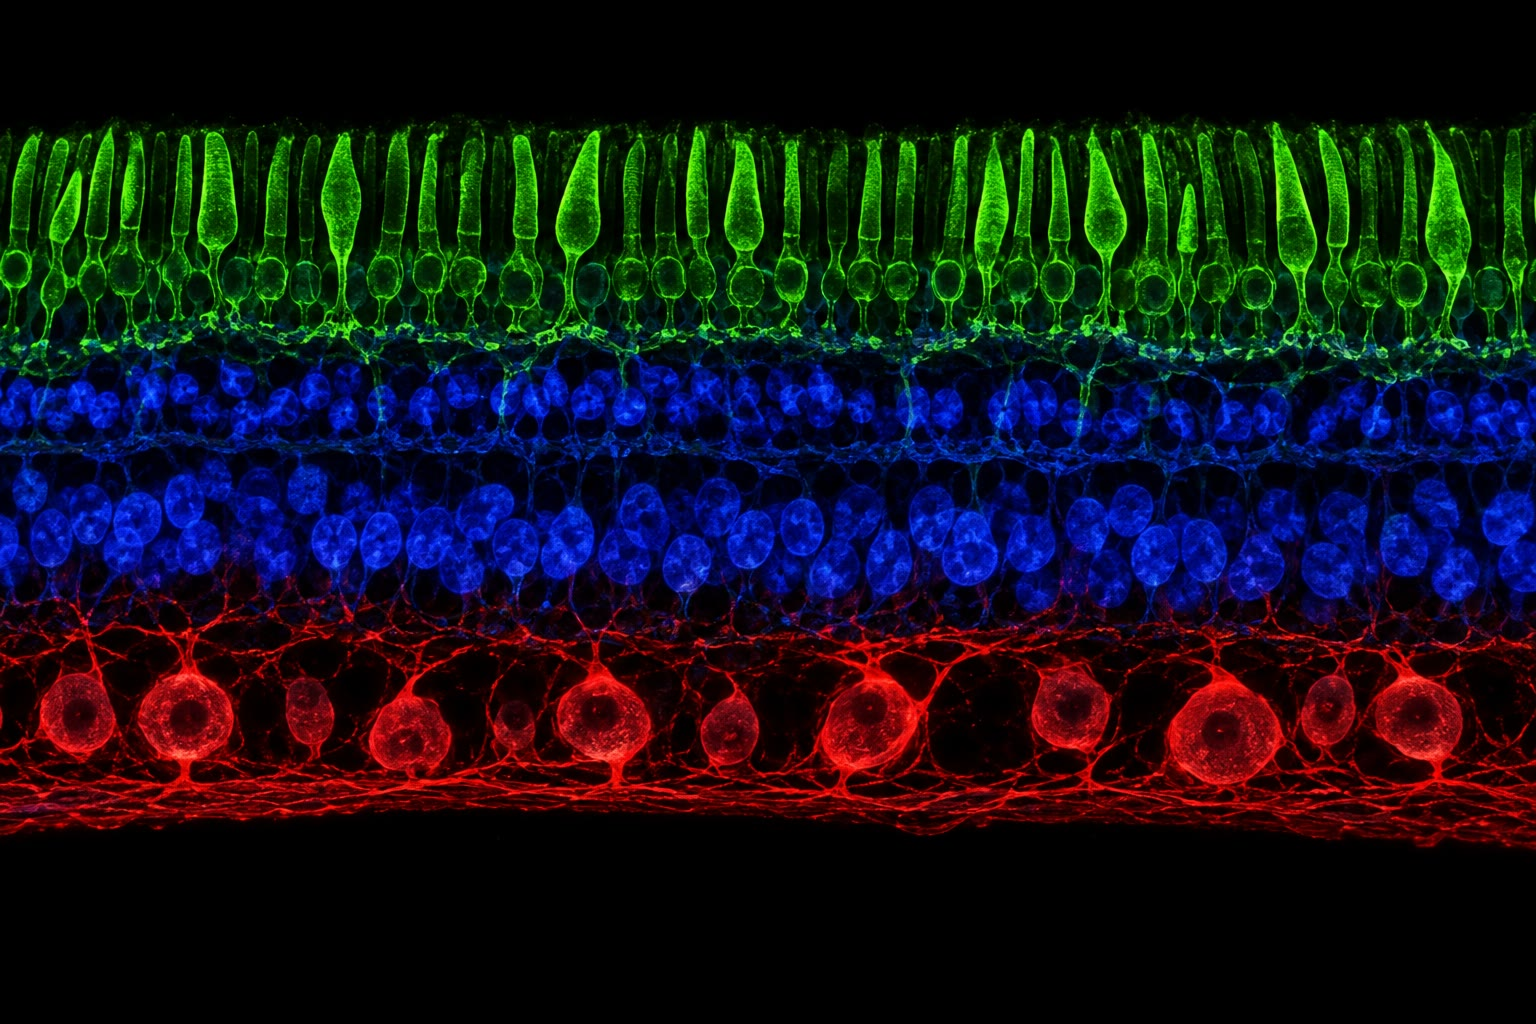
\includegraphics[width=0.46\linewidth]{images/book5/ai/b5-18-retina-section.jpg}\hspace{0.04\linewidth}
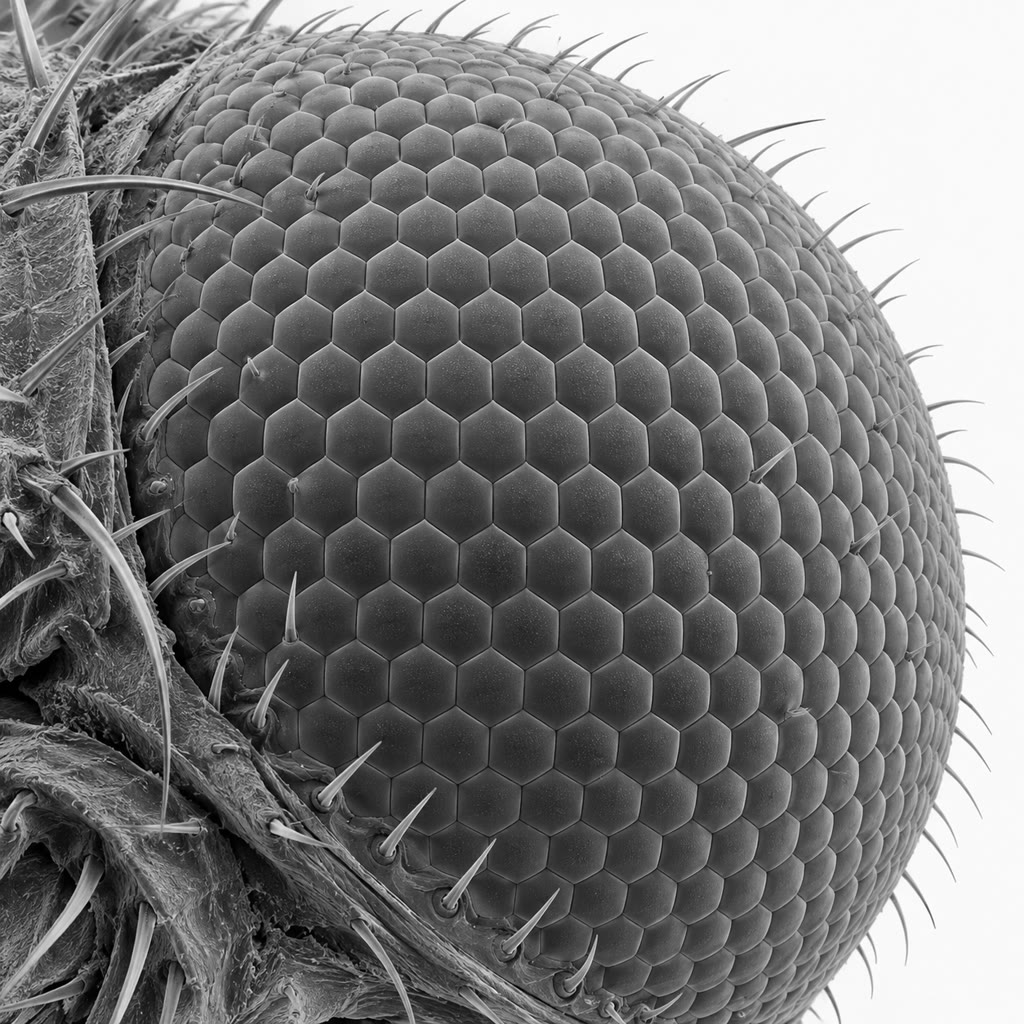
\includegraphics[width=0.36\linewidth]{images/book5/ai/b5-18-compound-eye.jpg}

{\small À gauche~: une coupe de la \omterm{def:b3:sensory-systems:retina}{rétine}, les photorécepteurs (en vert)
au fond, puis les cellules bipolaires et horizontales, puis les \omterm{def:b3:sensory-systems:retina}{cellules
ganglionnaires} (en rouge) dont les axones partent vers le cerveau. À
droite~: l'œil composé d'une mouche, des centaines de lentilles
distinctes ayant chacune ses récepteurs --- une autre solution au même
problème.}
\end{omfigure}

\section{L'audition et l'équilibre}

\begin{definition}[La cochlée]\label{def:b3:sensory-systems:cochlea}
\index{cochlée}\index{membrane basilaire}\index{tonotopie}\index{cellule ciliée}\index{stéréocils}\index{lien apical}\index{décibel}
Le son est une onde de pression~; le problème de l'oreille est de
détecter des variations de pression de quelques dizaines de
micropascals dans l'air et de les trier par fréquence. Le tympan et les
trois osselets de l'oreille moyenne concentrent la force des
\qty{55}{mm^2} du tympan sur les \qty{3}{mm^2} de la fenêtre ovale, ce
qui élève la pression d'un facteur vingt --- l'adaptation d'impédance
entre l'air et le liquide de l'oreille interne, sans laquelle le son se
réfléchirait presque tout entier. Dans la \emph{cochlée}, tube enroulé
long de \qty{35}{mm}, l'onde de pression chemine le long de la
\emph{membrane basilaire}, étroite et raide à la base, large et molle à
l'apex~; chaque fréquence fait vibrer la membrane le plus à un endroit
--- les hautes fréquences près de la base, les basses près de l'apex ---
une carte \emph{tonotopique} que le cerveau lit comme la hauteur du son.
Sur la membrane siègent les \emph{cellules ciliées}~: \num{3500}
cellules ciliées internes sur un seul rang, chacune couronnée d'un
faisceau de \emph{stéréocils} joints de pointe à pointe par de fins
\emph{liens apicaux}~; incliner le faisceau vers son cil le plus haut
étire les liens et ouvre des canaux cationiques en quelques
microsecondes, sans aucun second messager, et le potassium entre depuis
l'endolymphe, dont la composition inhabituelle et le potentiel de
$+\qty{80}{mV}$ donnent une force motrice de \qty{150}{mV}. Les cellules
ciliées internes renseignent le nerf auditif~; les \num{12000} cellules
ciliées externes, mues par le même mouvement, se contractent et
s'allongent avec le son grâce à la protéine motrice prestine et
réinjectent de l'énergie dans la vibration de la membrane --- un
amplificateur qui affine l'accord d'un facteur cent et dont la panne
fait la plupart des surdités. L'intensité se mesure en
\emph{décibels}~: $L = 10\log_{10}
(I/I_{0})$, avec $I_{0} = \qty{1e-12}{W/m^2}$ le seuil d'audition~;
l'oreille travaille sur \qty{120}{dB}, un facteur mille milliards en
intensité.
\end{definition}

\begin{omfigure}
\begin{tikzpicture}[every node/.style={font=\scriptsize}, >=stealth]
  % unrolled cochlea
  \begin{scope}
    \draw[thick, omDef, fill=omDef!10] (0,0.9) -- (7,1.4) -- (7,-1.4) -- (0,-0.9) -- cycle;
    \draw[very thick, omProp] (0,0.15) -- (7,-0.15); \draw[very thick, omProp] (0,-0.15) -- (7,0.15);
    \node[above] at (0.8,1.05) {base~: étroite, raide}; \node[above] at (6.2,1.5) {apex~: large, mou};
    \node[left, align=right] at (-0.1,0) {fenêtre ovale\\(depuis l'étrier)};
    \foreach \x/\f in {0.9/\qty{16}{kHz}, 2.3/\qty{4}{kHz}, 3.8/\qty{1}{kHz}, 5.4/\qty{250}{Hz}, 6.6/\qty{60}{Hz}} { \draw[omThm, thick] (\x,-0.55) -- (\x,0.55); \node[below, omThm] at (\x,-0.65) {\f}; }
    \node[below, align=center] at (3.5,-1.7) {membrane basilaire (en orange)~:\\chaque fréquence fait vibrer le plus\\un seul endroit --- la tonotopie};
  \end{scope}
  % hair cell mechanism
  \begin{scope}[xshift=8.2cm, yshift=-0.6cm]
    \draw[thick, fill=omMeth!20] (0,0) rectangle (1.6,1.2); \node[below] at (0.8,-0.05) {cellule ciliée};
    \foreach \x/\h in {0.35/0.6, 0.65/0.85, 0.95/1.1, 1.25/1.35} \draw[very thick, omMeth!70!black] (\x,1.2) -- (\x,1.2+\h);
    \foreach \x/\h/\xx/\hh in {0.35/0.6/0.65/0.85, 0.65/0.85/0.95/1.1, 0.95/1.1/1.25/1.35} \draw[omThm, thick] (\x,1.2+\h) -- (\xx,1.2+\hh-0.1);
    \draw[->, thick] (1.9,2.3) -- (2.4,2.3) node[right, align=left, font=\tiny] {incliner vers le plus haut~:\\les liens s'étirent,\\les canaux s'ouvrent en $\unit{\micro s}$~;\\K$^{+}$ entre (\qty{150}{mV})};
    \node[above, align=center] at (0.8,2.7) {stéréocils joints\\par des liens apicaux (en rouge)};
  \end{scope}
\end{tikzpicture}

{\small À gauche~: la \omterm{def:b3:sensory-systems:cochlea}{cochlée} déroulée --- la \omterm{def:b3:sensory-systems:cochlea}{membrane basilaire} passe
graduellement de raide à molle, et chaque fréquence culmine à sa propre
place. À droite~: un faisceau de cils, dont les liens apicaux ouvrent
mécaniquement les canaux de transduction quand le faisceau est incliné.}
\end{omfigure}

\begin{proof}[Faits expérimentaux]
Von Békésy (dans les années 1940) ouvrit les \omterm{def:b3:sensory-systems:cochlea}{cochlées} de cadavres,
saupoudra de particules d'argent la \omterm{def:b3:sensory-systems:cochlea}{membrane basilaire} et observa sous
une lumière stroboscopique des sons purs installer une onde progressive
dont le sommet se tenait d'autant plus près de la base que le son était
aigu --- le code de place, qui lui valut le prix Nobel en 1961.
Hudspeth (dans les années 1980) poussa un faisceau de cils unique avec
une fibre de verre et enregistra le courant~: il coulait en moins de
\qty{10}{\micro s} après la poussée, bien trop vite pour une cascade
enzymatique, proportionnellement au déplacement du faisceau vers son
rang le plus haut, et il disparaissait quand on coupait les liens
apicaux avec un chélateur du calcium. L'ouverture est mécanique --- le
lien tire le canal --- et c'est pourquoi l'audition est le plus rapide
des sens et pourquoi son transducteur est détruit par les sons forts qui
rompent les liens.
\end{proof}

\begin{example}[Les nombres de l'oreille]\label{ex:b3:sensory-systems:ear-numbers}
Au seuil d'audition la \omterm{def:b3:sensory-systems:cochlea}{membrane basilaire} bouge d'environ \qty{0.1}{nm}
et l'amplitude de pression vaut \qty{20}{\micro Pa}, deux milliardièmes
de la pression atmosphérique~; à \qty{120}{dB} la pression est un
million de fois plus grande et le mouvement de la membrane de quelques
dizaines de nanomètres. Une oreille jeune entend de \qty{20}{Hz} à
\qty{20}{kHz} et sépare des sons distants de \qty{0.3}{\%}, la
discrimination du code de place étant affinée par les \omterm{def:b3:sensory-systems:cochlea}{cellules ciliées}
externes. Les \num{30000} fibres du nerf auditif déchargent en phase
avec l'onde de pression jusqu'à environ \qty{4}{kHz} (le verrouillage de
phase), portant le temps à quelques dizaines de microsecondes près, d'où
le cerveau calcule la direction d'un son à partir de l'écart d'arrivée
aux deux oreilles --- aussi peu que \qty{10}{\micro s}. Les organes de
l'équilibre emploient les mêmes \omterm{def:b3:sensory-systems:cochlea}{cellules ciliées}~: dans les \emph{canaux
semi-circulaires} l'inertie du liquide les incline quand la tête tourne
(accélération angulaire), et dans les organes otolithiques une couche de
cristaux de carbonate de calcium les charge de la pesanteur et de
l'accélération linéaire.
\end{example}

\begin{omfigure}
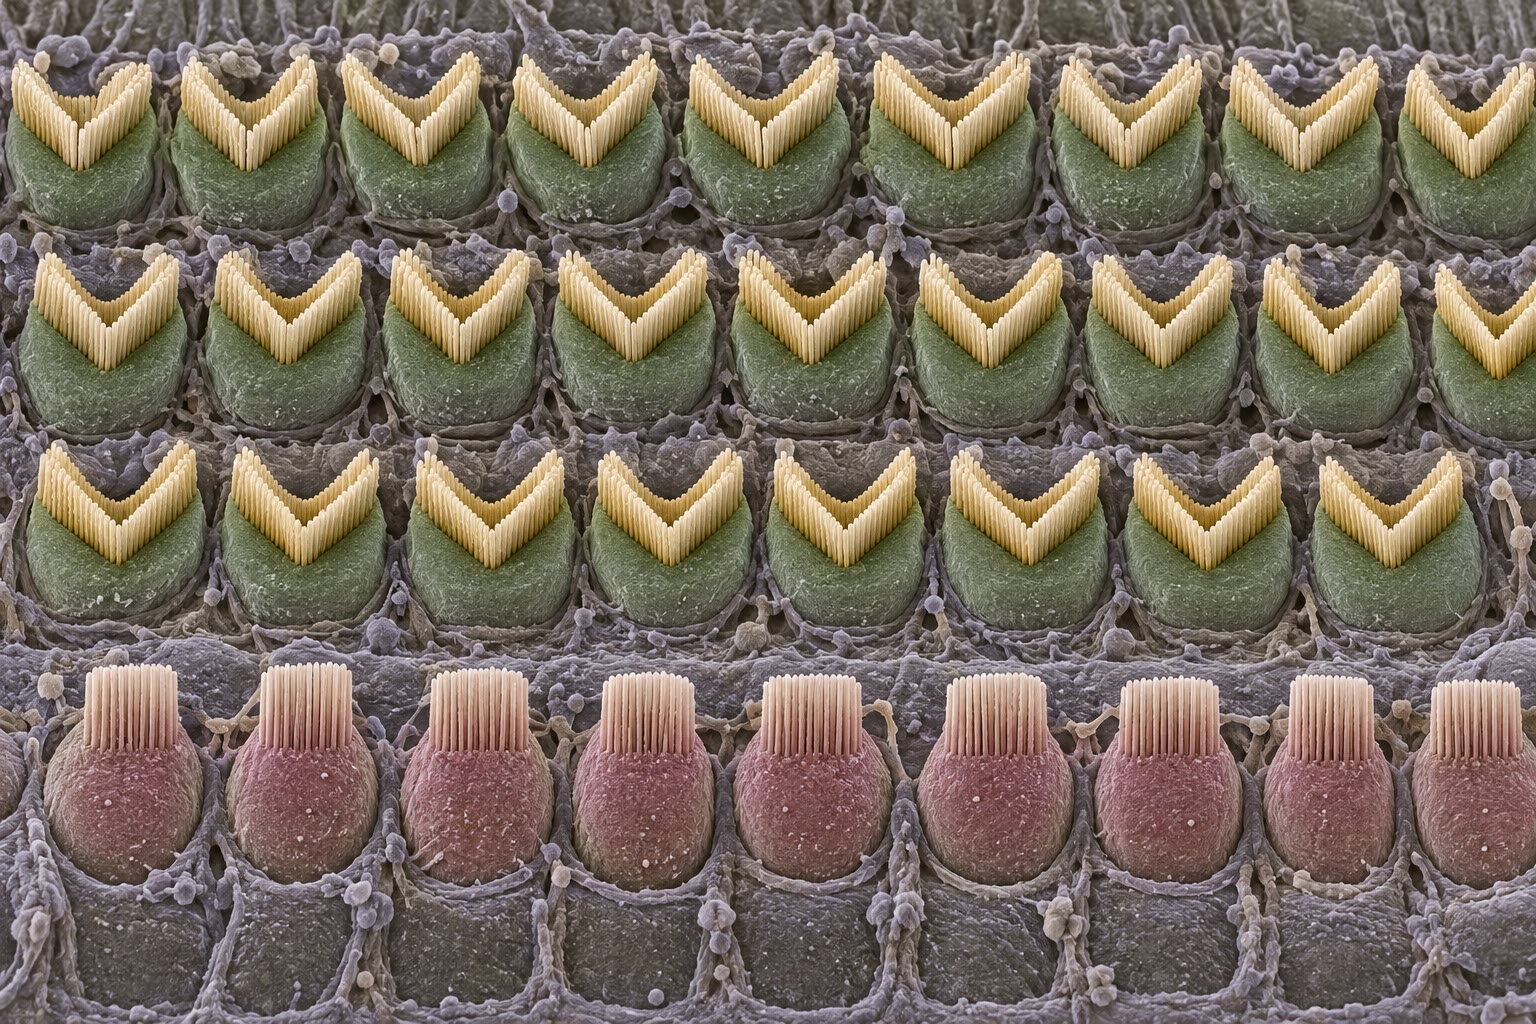
\includegraphics[width=0.54\linewidth]{images/book5/ai/b5-18-cochlea-hair-cells.jpg}

{\small L'organe de Corti vu de dessus~: trois rangs de \omterm{def:b3:sensory-systems:cochlea}{cellules ciliées}
externes à faisceaux en V, un rang de \omterm{def:b3:sensory-systems:cochlea}{cellules ciliées} internes. Les
liens apicaux de chaque faisceau ouvrent les canaux~; les cellules
externes amplifient, les internes rapportent.}
\end{omfigure}

\section{Les sens chimiques}

\begin{definition}[L'olfaction et le goût]\label{def:b3:sensory-systems:chemical}
\index{récepteur olfactif}\index{code combinatoire}\index{glomérule}\index{goût}
L'odorat commence dans une plage d'épithélium au sommet du nez, où
quelque dix millions de \emph{neurones sensoriels olfactifs} expriment
chacun un seul gène de \emph{récepteur olfactif} parmi environ $400$
chez l'humain (\num{1100} chez la souris, la plus grande famille de
gènes de l'un et l'autre génome) --- des récepteurs couplés aux
protéines~G qui lient des molécules odorantes dans une poche et, par
l'AMP cyclique, ouvrent un canal. Chaque récepteur lie plusieurs
odorants et chaque odorant lie plusieurs récepteurs, de sorte qu'une
odeur est un \emph{code combinatoire}, un motif d'activité sur les $400$
types de récepteurs, et qu'un carbone de plus dans une molécule change
le motif et l'odeur. Tous les neurones qui expriment un même récepteur
envoient leurs axones aux mêmes un ou deux \emph{glomérules} du bulbe
olfactif, de sorte que le bulbe porte une carte où chaque odeur est un
motif spatial de glomérules actifs, lue par le cortex sans passer par le
\omterm{def:b3:nervous-systems:plan}{thalamus}. Le goût est plus simple~: cinq modalités, chacune une \omterm{def:b3:sensory-systems:principles}{ligne
étiquetée} partant de ses propres cellules réceptrices --- le sucré,
l'umami et l'amer par des récepteurs couplés aux protéines~G (un
récepteur du sucré, un de l'umami, quelque vingt-cinq de l'amer), le
salé par un canal sodique, l'acide par un canal à protons --- et tout le
reste de ce que nous appelons la saveur est de l'odorat, qui gagne le
nez par le fond de la bouche.
\end{definition}

\begin{proof}[Faits expérimentaux]
Buck et Axel (1991) raisonnèrent que les récepteurs des odorants
seraient des récepteurs couplés aux protéines~G exprimés seulement dans
l'épithélium olfactif, et trouvèrent par PCR avec des \omterm{def:b3:genetic-engineering:pcr}{amorces}
dégénérées une famille de centaines de tels gènes, exprimés là et nulle
part ailleurs --- les récepteurs de l'odorat, inconnus depuis un siècle.
L'hybridation in situ montra un récepteur par neurone et la convergence
des neurones semblables sur des \omterm{def:b3:sensory-systems:chemical}{glomérules} uniques~; Malnic, Buck et
leurs collègues (1999) enregistrèrent des neurones isolés et montrèrent
que chaque odorant activait plusieurs types de récepteurs et chaque
récepteur plusieurs odorants --- le \omterm{def:b3:sensory-systems:chemical}{code combinatoire}. Bushdid et ses
collègues (2014) demandèrent à des sujets de discriminer des mélanges et
estimèrent que les humains distinguent plus de mille milliards d'odeurs,
bien au-delà des quelques milliers de la croyance commune.
\end{proof}

\begin{proposition}[La capacité d'un code combinatoire]\label{prop:b3:sensory-systems:combinatorial}
\index{code combinatoire!capacité}
Avec $R$ types de récepteurs chacun actif ou silencieux, une odeur peut
être représentée par l'un quelconque de $2^{R}$ motifs~; avec $R = 400$
cela fait $10^{120}$, et même en ne considérant que les motifs à
exactement $10$ types actifs il y en a
$\binom{400}{10} \approx 3\times 10^{20}$. La discrimination est limitée
non par le code mais par le bruit des récepteurs et par la lecture du
cerveau~: un code en \omterm{def:b3:sensory-systems:principles}{lignes étiquetées} à un récepteur par odeur
autoriserait $400$ odeurs, un \omterm{def:b3:sensory-systems:chemical}{code combinatoire} en autorise plus qu'il
n'y a de molécules à sentir. Le prix est qu'un récepteur isolé dit peu
de chose au cerveau~; le motif doit être lu comme un tout, ce que font
la carte glomérulaire et le cortex olfactif.
\end{proposition}

\begin{omfigure}
\begin{tikzpicture}[every node/.style={font=\scriptsize}, >=stealth]
  % receptor rows, odorant columns
  \foreach \i/\lab in {1/récepteur A, 2/récepteur B, 3/récepteur C, 4/récepteur D, 5/récepteur E} \node[left] at (-0.1,-0.7*\i) {\lab};
  \foreach \j/\lab in {1/hexanol, 2/heptanol, 3/octanol, 4/limonène} \node[above, rotate=0] at (1.2*\j-0.6,-0.35) {\lab};
  \foreach \i/\j/\v in {1/1/100, 1/2/30, 2/1/60, 2/2/100, 2/3/50, 3/2/40, 3/3/100, 3/4/20, 4/3/70, 5/4/100, 1/4/30} \fill[omThm!\v] (1.2*\j-1.15,-0.7*\i-0.3) rectangle (1.2*\j-0.05,-0.7*\i+0.3);
  \foreach \i in {1,...,5} \foreach \j in {1,...,4} \draw[gray!50] (1.2*\j-1.15,-0.7*\i-0.3) rectangle (1.2*\j-0.05,-0.7*\i+0.3);
  \node[below, align=center] at (2.1,-4.1) {chaque odorant active un ensemble de récepteurs,\\chaque récepteur un ensemble d'odorants~:\\l'odeur est la colonne};
  % glomerular map
  \begin{scope}[xshift=9.2cm, yshift=-2.2cm]
    \draw[thick, omDef!60, fill=omDef!8] (0,0) ellipse (2.6 and 1.7); \node[above] at (0,1.75) {bulbe olfactif~: les glomérules};
    \foreach \p in {(-1.8,0.6),(-1.0,1.0),(-0.2,0.7),(0.8,1.0),(1.7,0.5),(-1.6,-0.4),(-0.6,-0.6),(0.4,-0.3),(1.3,-0.7),(0.1,0.2)} \draw[omDef!70, fill=omDef!25] \p circle (0.25);
    \fill[omThm!80] (-1.0,1.0) circle (0.25); \fill[omThm!50] (0.4,-0.3) circle (0.25); \fill[omThm!80] (1.7,0.5) circle (0.25);
    \node[below, align=center] at (0,-1.8) {tous les neurones d'un type de récepteur\\convergent sur un glomérule~: une odeur est\\un motif spatial (en rouge) que le cortex lit};
  \end{scope}
\end{tikzpicture}

{\small Le \omterm{def:b3:sensory-systems:chemical}{code combinatoire} de l'odorat. À gauche~: une matrice
récepteurs par odorants, où chaque odeur est un motif en colonne. À
droite~: le motif étalé sur les \omterm{def:b3:sensory-systems:chemical}{glomérules} du bulbe.}
\end{omfigure}

\begin{omfigure}
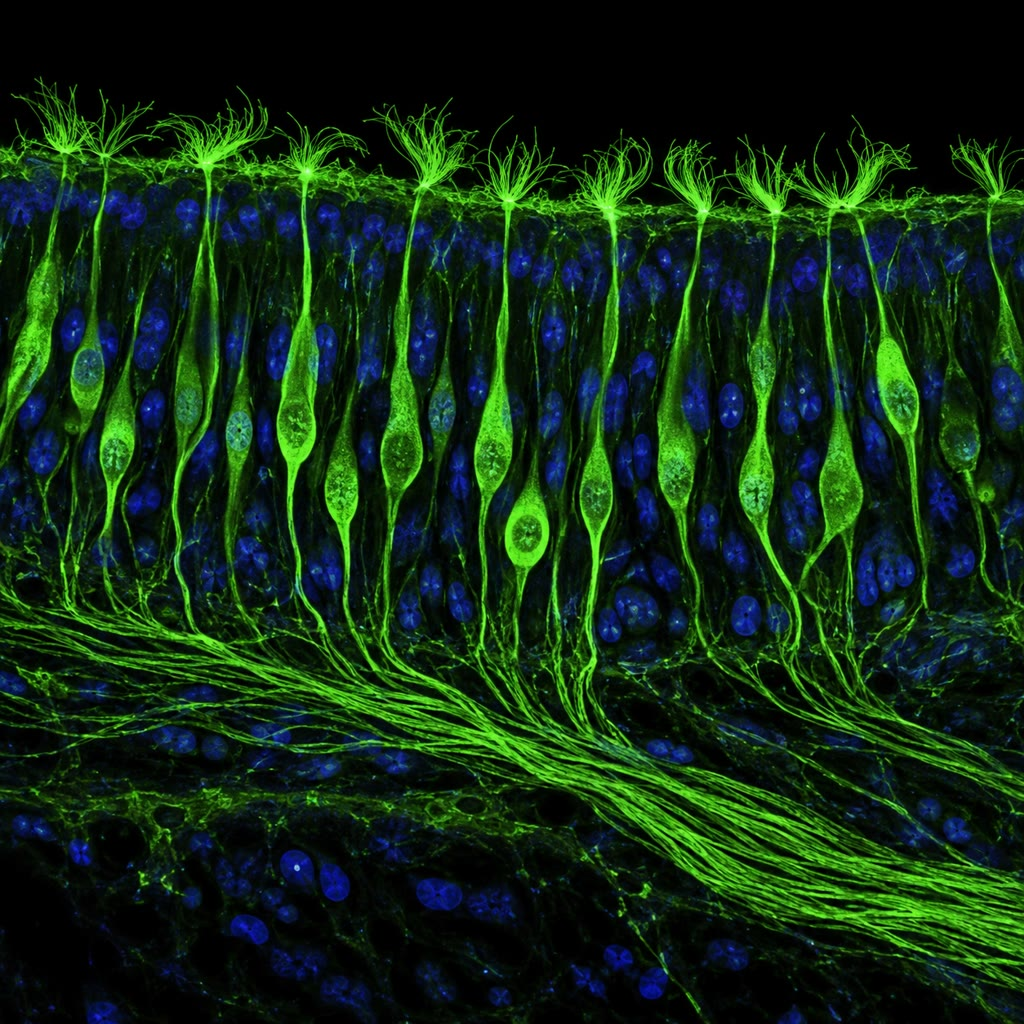
\includegraphics[width=0.40\linewidth]{images/book5/ai/b5-18-olfactory-epithelium.jpg}

{\small L'épithélium olfactif~: des neurones sensoriels (en vert) à
dendrites ciliées en surface, où se lient les odorants, et des axones
qui se rassemblent en dessous vers le bulbe. Chaque neurone exprime un
seul gène de récepteur sur les quatre cents.}
\end{omfigure}

\section{Le toucher, la température, la douleur et les sens qui nous manquent}

\begin{definition}[La somesthésie]\label{def:b3:sensory-systems:somato}
\index{mécanorécepteur}\index{canal Piezo}\index{canal TRP}\index{nocicepteur}\index{proprioception}
La peau porte plusieurs sortes de \emph{mécanorécepteurs}, chacun un
axone se terminant dans sa propre capsule~: les cellules de Merkel pour
la pression fine et la texture (adaptation lente, petits champs), les
corpuscules de Meissner pour le toucher léger et le glissement
(adaptation rapide), les corpuscules de Pacini profonds dans la peau
pour la vibration (adaptation très rapide, champs énormes), les
terminaisons de Ruffini pour l'étirement. Le transducteur de la plupart
d'entre eux est \emph{Piezo2}, un canal ionique géant à hélice de pales
qui s'ouvre quand la membrane est étirée~; sans lui le toucher et le
sens de la position du corps sont perdus, et le même canal dans les
poumons et la vessie en sent le remplissage. La \emph{température} est
perçue par des canaux de la famille TRP accordés à différentes plages
--- TRPV1, ouvert par la chaleur au-dessus de \qty{43}{\celsius} et par
la capsaïcine, et c'est pourquoi le piment «~brûle~»~; TRPM8, ouvert par
le froid et par le menthol --- et la \emph{douleur} par des
terminaisons nerveuses libres, les \emph{nocicepteurs}, qui répondent à
une chaleur, une pression ou des substances chimiques nocives (protons,
ATP, bradykinine) et dont les seuils sont abaissés par l'\omterm{def:b3:innate-immunity:inflammation}{inflammation}
(\cref{ch:b3:innate-immunity}). La \emph{proprioception}, le sens de
l'endroit où sont les membres, vient des fuseaux neuromusculaires et des
organes tendineux du \cref{ch:b3:nervous-systems} et de Piezo2 dans les
capsules articulaires. La densité des récepteurs fixe l'acuité~: deux
points distants de \qty{2}{mm} se distinguent sur le bout du doigt, il
en faut \qty{40}{mm} dans le dos.
\end{definition}

\begin{method}[Mesurer un sens]\label{met:b3:sensory-systems:psychophysics}
\index{psychophysique}\index{seuil}\index{discrimination de deux points}
Pour caractériser un canal sensoriel~: (1) trouver le \emph{seuil
absolu} en présentant de nombreuses fois des stimulus d'intensité
graduée et en ajustant la fraction détectée --- l'intensité détectée une
fois sur deux --- comme le fit Hecht~; (2) trouver le \emph{seuil
différentiel} à plusieurs intensités et vérifier la \omterm{thm:b3:sensory-systems:weber}{loi de Weber}~; (3)
cartographier l'\emph{acuité spatiale} avec deux stimulus à écartement
variable (le test des deux points sur la peau, un réseau sur la
\omterm{def:b3:sensory-systems:retina}{rétine})~; (4) cartographier l'\emph{acuité temporelle} avec un
scintillement ou des clics (un scintillement fusionne vers \qty{60}{Hz}
en vision diurne)~; (5) chez un animal, enregistrer des fibres
afférentes isolées en appliquant les mêmes stimulus et comparer les
seuils neuronaux aux seuils comportementaux --- la psychophysique et la
physiologie devraient s'accorder, et là où elles ne s'accordent pas
l'écart est ce que le cerveau ajoute.
\end{method}

\begin{remark}[D'autres animaux, d'autres sens]\label{rem:b3:sensory-systems:others}
Chaque sens vu ici a une version qu'un animal a poussée plus loin, et il
est des sens qui nous manquent. Requins et raies perçoivent les champs
de quelques microvolts des battements de cœur d'une proie par des canaux
remplis de gelée~; les poissons électriques lisent les déformations de
leur propre champ pour voir dans le noir. Les crotales imagent en
infrarouge les proies chaudes grâce à leurs fossettes~; chauves-souris
et dauphins écholocalisent, chronométrant à quelques microsecondes les
échos de leurs propres cris et pilotant la fréquence du cri pour suivre
un papillon~; les abeilles voient l'ultraviolet et la polarisation de la
lumière du ciel et s'y orientent~; les oiseaux migrateurs et les tortues
perçoivent le champ magnétique terrestre par un mécanisme encore
discuté. Le nez d'un chien a quarante fois nos neurones récepteurs et un
tiers de son cerveau pour les lire~; un hibou entend une souris sous la
neige. Les principes ne changent pas --- un transducteur, une \omterm{def:b3:sensory-systems:principles}{ligne
étiquetée}, un code, une compression, une carte --- et la variété est ce
que l'évolution en a fait.
\end{remark}

\section{Exercices}

\begin{exercise}[$\star$]\label{exo:b3:sensory-systems:1}
Expliquer comment le cerveau sait si un train de potentiels vient de
l'œil ou de l'oreille, alors que les potentiels sont identiques.
\end{exercise}

\begin{exercise}[$\star$]\label{exo:b3:sensory-systems:2}
Pourquoi la lumière hyperpolarise-t-elle un photorécepteur, et qu'est-ce
que le courant d'obscurité~?
\end{exercise}

\begin{exercise}[$\star$]\label{exo:b3:sensory-systems:3}
Un chuchotement fait \qty{20}{dB}, une conversation \qty{60}{dB}, un
concert de rock \qty{110}{dB}. Calculer l'intensité de chacun en
W/m$^{2}$ et le rapport entre le plus fort et le plus faible.
\end{exercise}

\begin{exercise}[$\star$]\label{exo:b3:sensory-systems:4}
Énoncer les cinq modalités du \omterm{def:b3:sensory-systems:chemical}{goût} et leurs types de récepteurs, et
expliquer pourquoi un rhume bloque le «~\omterm{def:b3:sensory-systems:chemical}{goût}~» des aliments.
\end{exercise}

\begin{exercise}[$\star\star$]\label{exo:b3:sensory-systems:5}
La fraction de Weber pour le poids vaut $0.02$. En partant d'un poids de
\qty{100}{g}, combien de pas juste perceptibles séparent celui-ci de
\qty{10}{kg}~? Utiliser la formule de Fechner et vérifier en comptant
des pas de facteur $1.02$.
\end{exercise}

\begin{exercise}[$\star\star$]\label{exo:b3:sensory-systems:6}
À l'aide du \cref{thm:b3:sensory-systems:hecht}, calculer
$P_{\text{vu}}$ pour $a = 2$, $6$ et $12$ photons absorbés avec un seuil
de $n = 6$. Pour quel $a$ l'éclair est-il vu une fois sur deux~? Si
\qty{10}{\%} des photons arrivant à la cornée sont absorbés, combien
l'éclair doit-il en délivrer~?
\end{exercise}

\begin{exercise}[$\star\star$]\label{exo:b3:sensory-systems:7}
L'oreille moyenne concentre la force de \qty{55}{mm^2} sur
\qty{3}{mm^2} avec un levier de $1.3$. De quel facteur la pression
est-elle élevée, et de combien de \omterm{def:b3:sensory-systems:cochlea}{décibels}~? Pourquoi l'oreille d'une
personne aux osselets soudés (otospongiose) est-elle plus sourde de
quelques dizaines de \omterm{def:b3:sensory-systems:cochlea}{décibels}~?
\end{exercise}

\begin{exercise}[$\star\star$]\label{exo:b3:sensory-systems:8}
Expliquer pourquoi le courant de transduction d'une \omterm{def:b3:sensory-systems:cochlea}{cellule ciliée}
apparaît en quelques microsecondes alors que celui d'un photorécepteur
prend des dizaines de millisecondes, et ce que chaque sens gagne à sa
conception.
\end{exercise}

\begin{exercise}[$\star\star$]\label{exo:b3:sensory-systems:9}
Une souris a \num{1100} types de récepteurs et un humain $400$. Si une
odeur active environ \qty{5}{\%} des types, combien de motifs
d'exactement cette taille sont disponibles pour chacun (utiliser
$\binom{R}{k}$ avec $k = 0.05R$, et l'approximation de Stirling
$\ln\binom{R}{k} \approx R\,H(k/R)$ avec
$H(p) = -p\ln p - (1-p)\ln(1-p)$)~?
\end{exercise}

\begin{exercise}[$\star\star\star$]\label{exo:b3:sensory-systems:10}
Un \omterm{def:b3:sensory-systems:retina}{bâtonnet} isomérise spontanément une \omterm{def:b3:sensory-systems:retina}{rhodopsine} toutes les
\qty{40}{s} dans le noir. Dans une plage de $500$ \omterm{def:b3:sensory-systems:retina}{bâtonnets} observée
pendant une fenêtre de \qty{0.1}{s}, quel est le nombre moyen
d'événements spontanés, et la probabilité qu'il s'en produise six ou
plus par hasard~? Expliquer pourquoi le cerveau met le seuil vers six et
non à un.
\end{exercise}

\begin{exercise}[$\star\star\star$]\label{exo:b3:sensory-systems:11}
Le nerf auditif verrouille ses potentiels sur la phase du son jusqu'à
\qty{4}{kHz}, avec une gigue d'environ \qty{20}{\micro s}. Le son voyage
à \qty{340}{m/s} et les oreilles sont distantes de \qty{20}{cm}. Quel
est le plus grand délai interaural, quelle résolution angulaire une
discrimination de \qty{10}{\micro s} donne-t-elle près du plan médian,
et pourquoi le code de place, et non le temps, sert-il au-dessus de
\qty{4}{kHz}~?
\end{exercise}

\begin{exercise}[$\star\star\star$]\label{exo:b3:sensory-systems:12}
L'\omterm{def:b3:sensory-systems:principles}{inhibition latérale} fait paraître plus clair, au bord, un champ gris
uniforme voisin d'un champ sombre. Modéliser une rangée de récepteurs
excités chacun par sa propre lumière $I_{i}$ et inhibés par une fraction
$w$ de celle de chaque voisin, $r_{i} = I_{i} - w(I_{i-1} + I_{i+1})$,
et calculer la réponse en travers d'une marche de $I = 1$ à $I = 2$ avec
$w = 0.2$. Qu'y gagne et qu'y perd la \omterm{def:b3:sensory-systems:retina}{rétine}~?
\end{exercise}

\section{Problème~: une bougie vue de loin}

\begin{problem}[{Problème du week-end --- les photons d'une bougie
comptés dans un œil lointain, la détection de l'éclair calculée par la
statistique de Poisson et l'amplificateur du bâtonnet, les décibels d'un
concert convertis en mouvement du tympan et en courant de cellule
ciliée, et le code d'un nez dénombré, pour finir sur la distance à
laquelle la bougie est vue, la pression au tympan et les motifs qu'un
nez peut former}]
\label{pb:b3:sensory-systems:1}
Données~: une bougie émet environ \qty{0.01}{W} de lumière visible, à
\qty{550}{nm} (énergie du photon $3.6\times 10^{-19}$ J). Une pupille
adaptée au noir fait \qty{7}{mm} de diamètre~; \qty{10}{\%} des photons
entrant dans l'œil sont absorbés par la \omterm{def:b3:sensory-systems:retina}{rhodopsine}~; l'œil intègre sur
\qty{0.1}{s}~; le seuil est de $6$ photons absorbés. Chaque photon
absorbé ferme $200$ canaux et réduit le courant d'obscurité de
\qty{1}{pA} pendant \qty{0.2}{s}~; le courant d'obscurité d'un \omterm{def:b3:sensory-systems:retina}{bâtonnet}
vaut \qty{30}{pA}. Son~: $I_{0} =
\qty{1e-12}{W/m^2}$~; le tympan a une aire de \qty{55}{mm^2}~; un
faisceau de cils de \qty{5}{\micro m} de haut se défléchit au seuil de
\qty{0.3}{nm}. Olfaction~: $R = 400$ récepteurs~; le courant de
transduction d'une \omterm{def:b3:sensory-systems:cochlea}{cellule ciliée} vaut \qty{100}{pA} à saturation.

\medskip
\noindent\textbf{Partie I --- Les photons.}
\begin{enumerate}
  \item Combien de photons par seconde la bougie émet-elle~?
  \item À la distance $d$ les photons sont répartis sur une sphère
        d'aire $4\pi d^{2}$. Combien entrent dans la pupille par seconde
        à \qty{1}{km}~? À \qty{10}{km}~?
  \item Combien en sont absorbés dans une fenêtre d'intégration à chaque
        distance~? La bougie est-elle vue (seuil $6$)~?
  \item Trouver la distance à laquelle le nombre moyen absorbé dans une
        fenêtre vaut $6$. Avec la statistique de Poisson, quelle
        fraction des fenêtres y dépasse le seuil~?
  \item À la distance de la question 4, quelle est la probabilité qu'une
        fenêtre de \qty{0.1}{s} donnée ne contienne aucun photon~?
        Pourquoi une étoile faible semble-t-elle scintiller~?
  \item Sous la pleine lune les mêmes \omterm{def:b3:sensory-systems:retina}{bâtonnets} absorbent $10^{4}$
        photons du ciel par fenêtre. Expliquer pourquoi la bougie à
        \qty{10}{km} est alors invisible bien qu'elle délivre les mêmes
        photons.
\end{enumerate}

\medskip
\noindent\textbf{Partie II --- L'amplificateur du \omterm{def:b3:sensory-systems:retina}{bâtonnet}.}
\begin{enumerate}[resume]
  \item Un photon ferme $200$ canaux et réduit le courant de
        \qty{1}{pA}. Quel courant porte un canal, et combien de cations
        par seconde cela fait-il ($e = \qty{1.6e-19}{C}$)~?
  \item Quelle fraction du courant d'obscurité un photon retire-t-il~?
        Combien de photons simultanés éteindraient complètement le
        \omterm{def:b3:sensory-systems:retina}{bâtonnet} (saturation)~?
  \item La réponse dure \qty{0.2}{s}. Combien de cations un photon
        empêche-t-il d'entrer~? Quel est le gain en charge par photon~?
  \item En plein jour $10^{5}$ photons par seconde atteignent un
        \omterm{def:b3:sensory-systems:retina}{bâtonnet}. Que lui arrive-t-il, et pourquoi les \omterm{def:b3:sensory-systems:retina}{cônes}, qui
        s'adaptent et saturent moins, sont-ils les récepteurs du jour~?
  \item Les \omterm{def:b3:sensory-systems:retina}{cônes} ont besoin d'environ $100$ photons pour signaler.
        Expliquer, en termes d'arbitrage entre sensibilité et rapidité,
        pourquoi les \omterm{def:b3:sensory-systems:retina}{cônes} répondent en \qty{20}{ms} et les \omterm{def:b3:sensory-systems:retina}{bâtonnets} en
        \qty{200}{ms}.
  \item Une \omterm{def:b3:sensory-systems:retina}{rhodopsine} s'isomérise spontanément une fois toutes les
        \qty{40}{s}. Sur les $10^{8}$ \omterm{def:b3:sensory-systems:retina}{bâtonnets} d'un œil, combien de
        faux photons par seconde la \omterm{def:b3:sensory-systems:retina}{rétine} engendre-t-elle, et pourquoi
        cela n'aveugle-t-il pas de bruit l'œil dans le noir~? (Penser au
        seuil et au \omterm{def:b3:sensory-systems:principles}{champ récepteur}.)
\end{enumerate}

\medskip
\noindent\textbf{Partie III --- Les \omterm{def:b3:sensory-systems:cochlea}{décibels}.}
\begin{enumerate}[resume]
  \item Un concert à \qty{110}{dB}~: intensité en W/m$^{2}$ et puissance
        tombant sur un tympan.
  \item Quelle énergie acoustique le tympan reçoit-il pendant un concert
        de deux heures~? Comparer à l'énergie d'une goutte de pluie qui
        tombe (\qty{1e-4}{J}).
  \item Le seuil d'audition à \qty{0}{dB}~: puissance sur le tympan et
        énergie par \qty{10}{ms} --- comparer à l'énergie d'un photon
        visible.
  \item Le faisceau de cils se défléchit de \qty{0.3}{nm} au seuil sur
        une hauteur de \qty{5}{\micro m}. Quel angle cela fait-il, en
        degrés~? Comparer la déflexion au diamètre d'un atome
        d'hydrogène (\qty{0.1}{nm}).
  \item Une exposition prolongée au-dessus de \qty{85}{dB} abîme les
        \omterm{def:b3:sensory-systems:cochlea}{cellules ciliées}, et les \omterm{def:b3:sensory-systems:cochlea}{cellules ciliées} ne se régénèrent pas
        chez les mammifères. Deux heures à \qty{110}{dB} délivrent autant
        d'énergie que combien d'heures à \qty{85}{dB}~?
  \item L'étendue de l'audition fait \qty{120}{dB}. Combien de pas juste
        perceptibles de force sonore cela fait-il, si la fraction de
        Weber pour l'intensité vaut environ $0.25$ (un \omterm{def:b3:sensory-systems:cochlea}{décibel})~?
\end{enumerate}

\medskip
\noindent\textbf{Partie IV --- Le code de l'odorat.}
\begin{enumerate}[resume]
  \item Avec $400$ récepteurs chacun allumé ou éteint, combien de
        motifs~? Écrire la réponse en puissance de dix.
  \item Si une odeur active d'ordinaire $20$ récepteurs, combien y
        a-t-il de motifs distincts de ce genre ($\binom{400}{20}$,
        utiliser Stirling ou les logarithmes)~?
  \item Deux odorants partagent $15$ de leurs $20$ récepteurs. Proposer
        une mesure de leur distance dans le code et expliquer pourquoi
        ils sentent pareil.
  \item Les humains discriminent environ mille milliards d'odeurs.
        Quelle fraction des motifs de la question 20 cela fait-il, et
        qu'est-ce qui limite ce nombre bien en dessous de la capacité du
        code~?
  \item Une souris à \num{1100} récepteurs~: combien de motifs de $20$
        de plus qu'un humain, en puissance de dix~?
  \item Une mutation supprime un gène de récepteur. Prévoir son effet
        sur la capacité à sentir en général et sur la perception d'un
        odorant qui lie fortement ce récepteur (une anosmie spécifique).
  \item Résumer~: la distance à laquelle la bougie est vue (question~4),
        l'énergie acoustique sur le tympan au seuil en \qty{10}{ms}
        (question~15), et le nombre de motifs à vingt récepteurs qu'un
        nez humain peut former (question~20).
\end{enumerate}
\end{problem}
